% !TeX root = ../main.tex

\section{Sviluppo Applicazione}

\begin{frame}{Processo di Sviluppo}
    \begin{columns}[onlytextwidth]
        \begin{column}{0.4\textwidth}
            \textbf{Progettazione}:
            \begin{itemize}
                \item Modellazione dominio (editoria digitale)
                \item Progettazione UX/UI
                \item Definizione architettura
            \end{itemize}
            \vspace{3mm}
            \textbf{Implementazione}:
            \begin{itemize}
                \item Ricerca Librerie
                \item Configurazione utilizzo sistema di automazione
                \item Sviluppo logica applicativa (modulo condiviso)
                \item Sviluppo UI Android
                \item Sviluppo UI iOS
            \end{itemize}
        \end{column}
        \begin{column}{0.6\textwidth}
             \begin{figure}[H]
                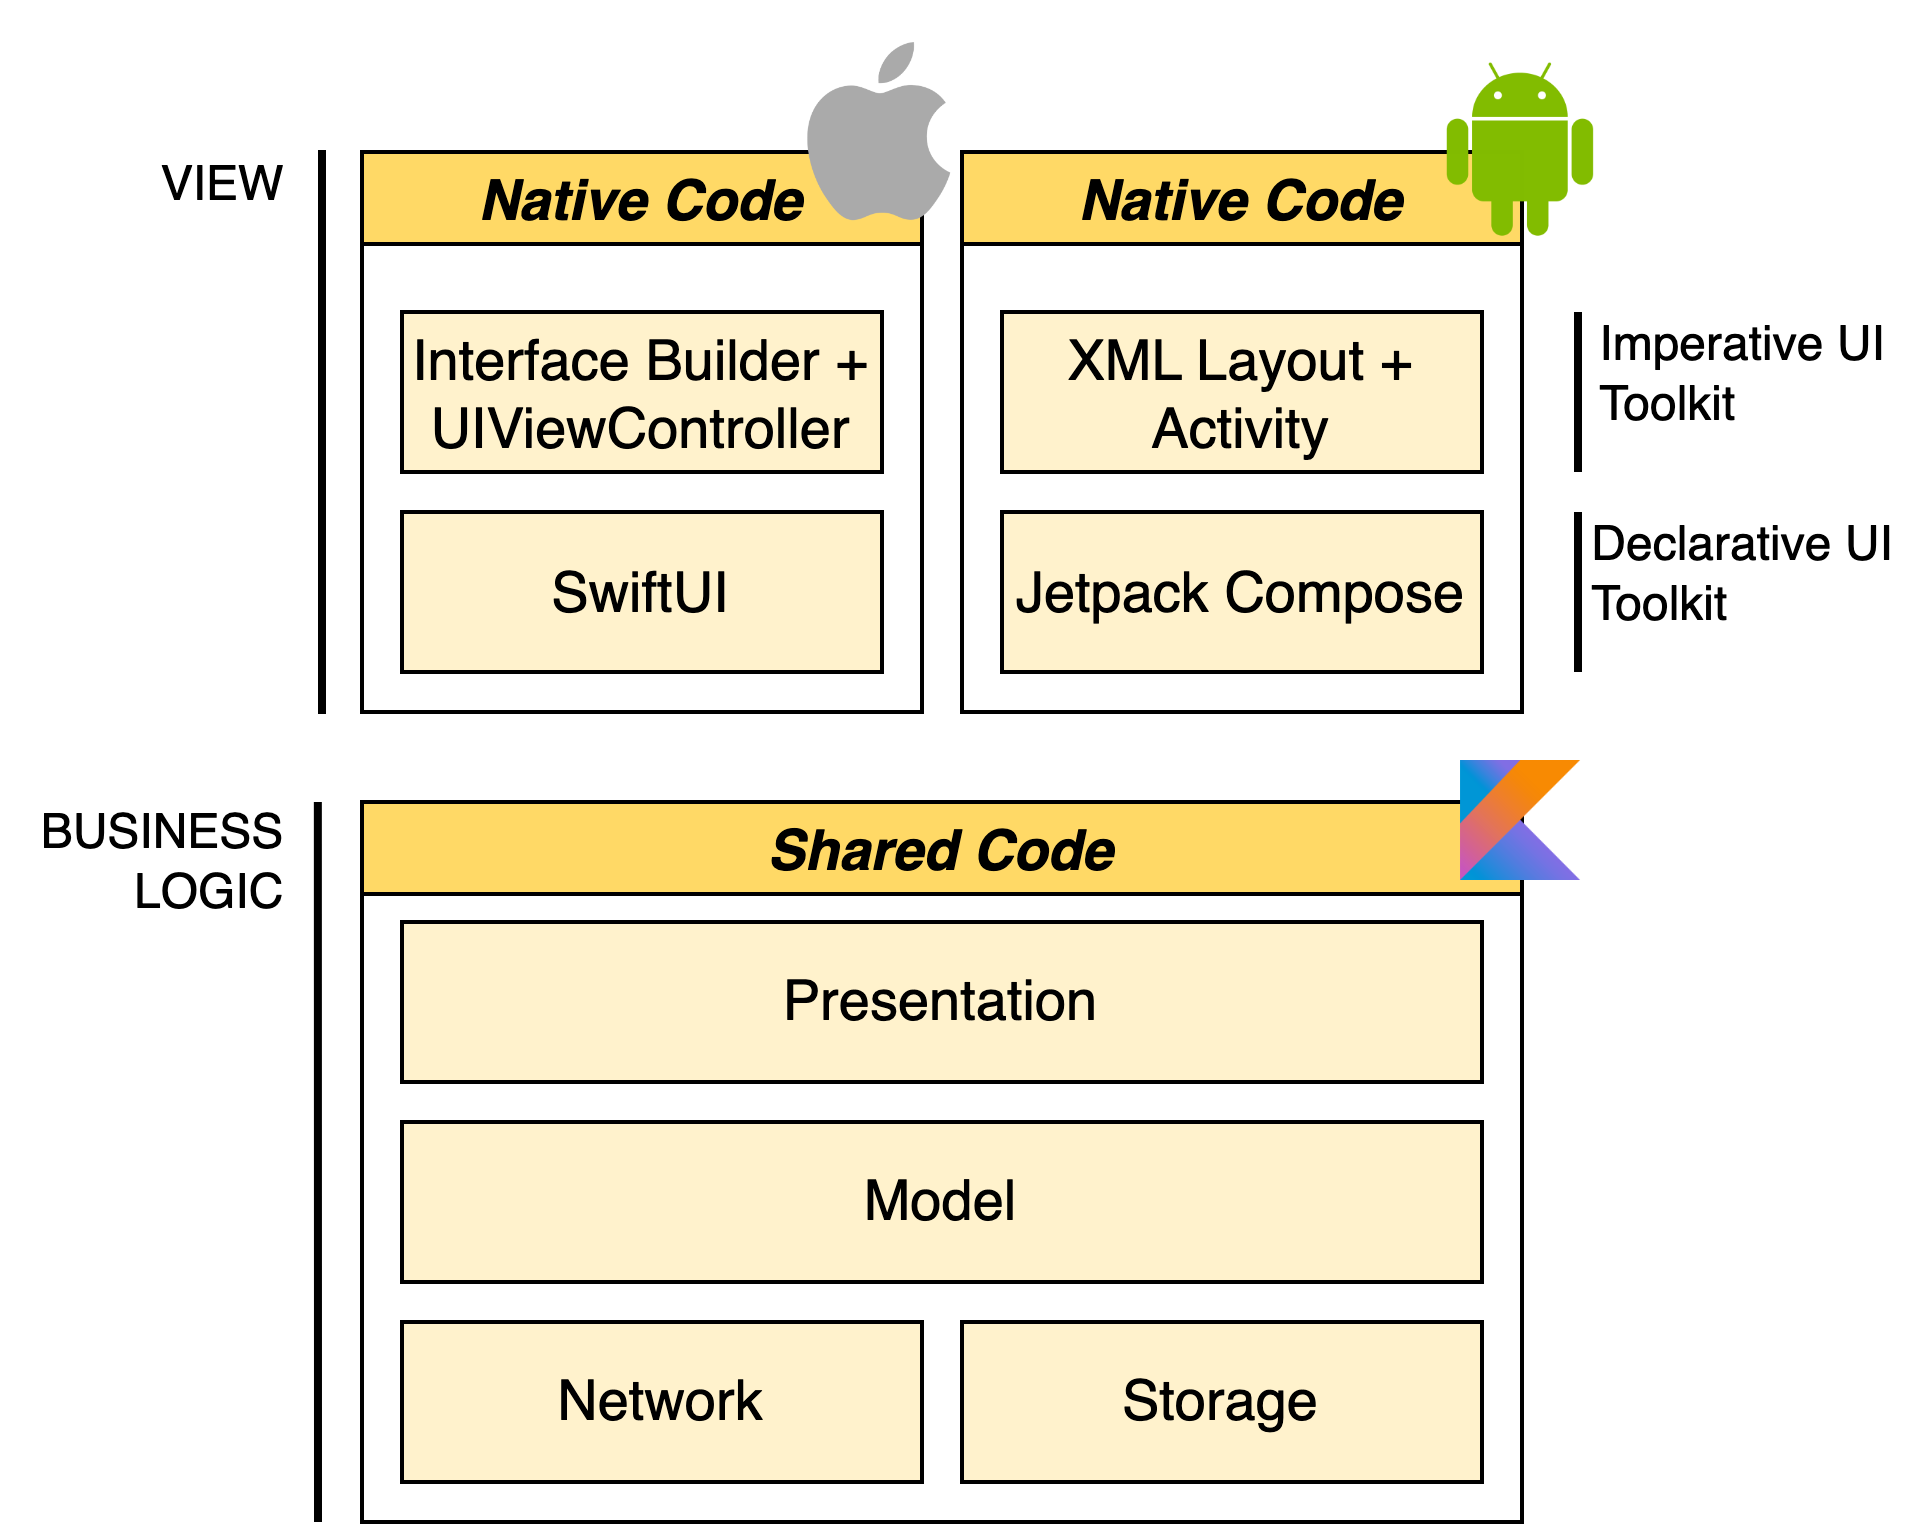
\includegraphics[width=1\textwidth]{img/stack_kmm.png}
            \end{figure}
        \end{column}
    \end{columns}
\end{frame}

\begin{frame}{Logica Applicativa}
    \begin{columns}[onlytextwidth]
        \begin{column}{0.4\textwidth}
            \textbf{Strategie}:
            \begin{itemize}
                \item Librerie di terze parti con supporto multipiattaforma
                \item Meccanismo ``expect/actual''
            \end{itemize}
        \end{column}
        \begin{column}{0.6\textwidth}
             \begin{figure}[H]
                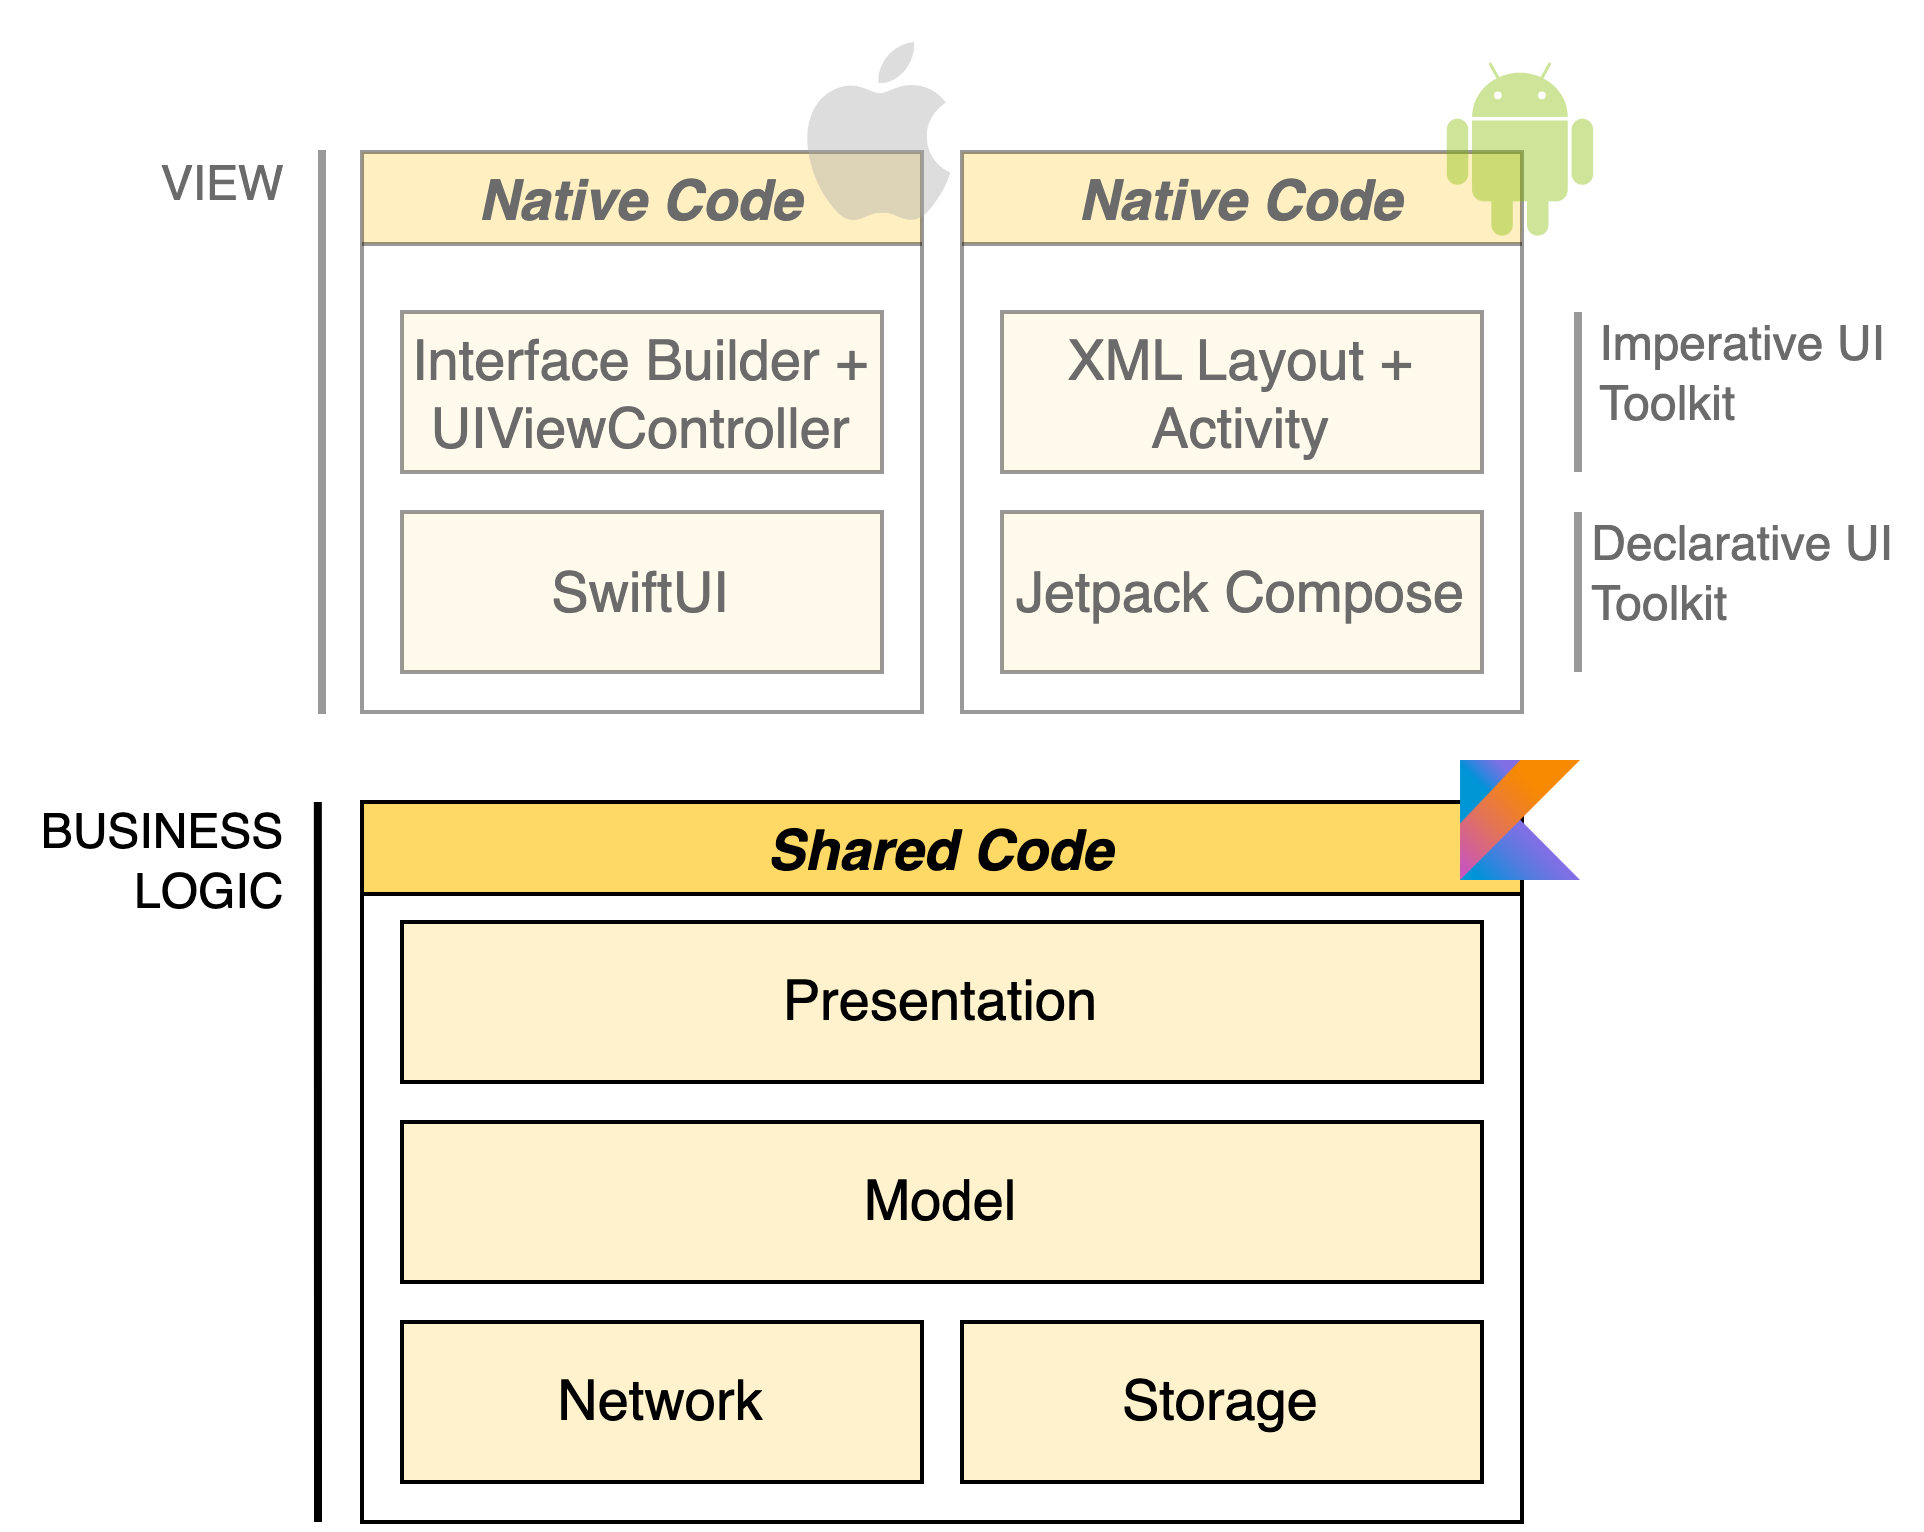
\includegraphics[width=1\textwidth]{img/stack_kmm_shared.png}
            \end{figure}
        \end{column}
    \end{columns}
\end{frame}

\begin{frame}{UI Android}
    % citare readium kotlin
    \begin{columns}[onlytextwidth]
        \begin{column}{0.4\textwidth}

        \end{column}
        \begin{column}{0.6\textwidth}
             \begin{figure}[H]
                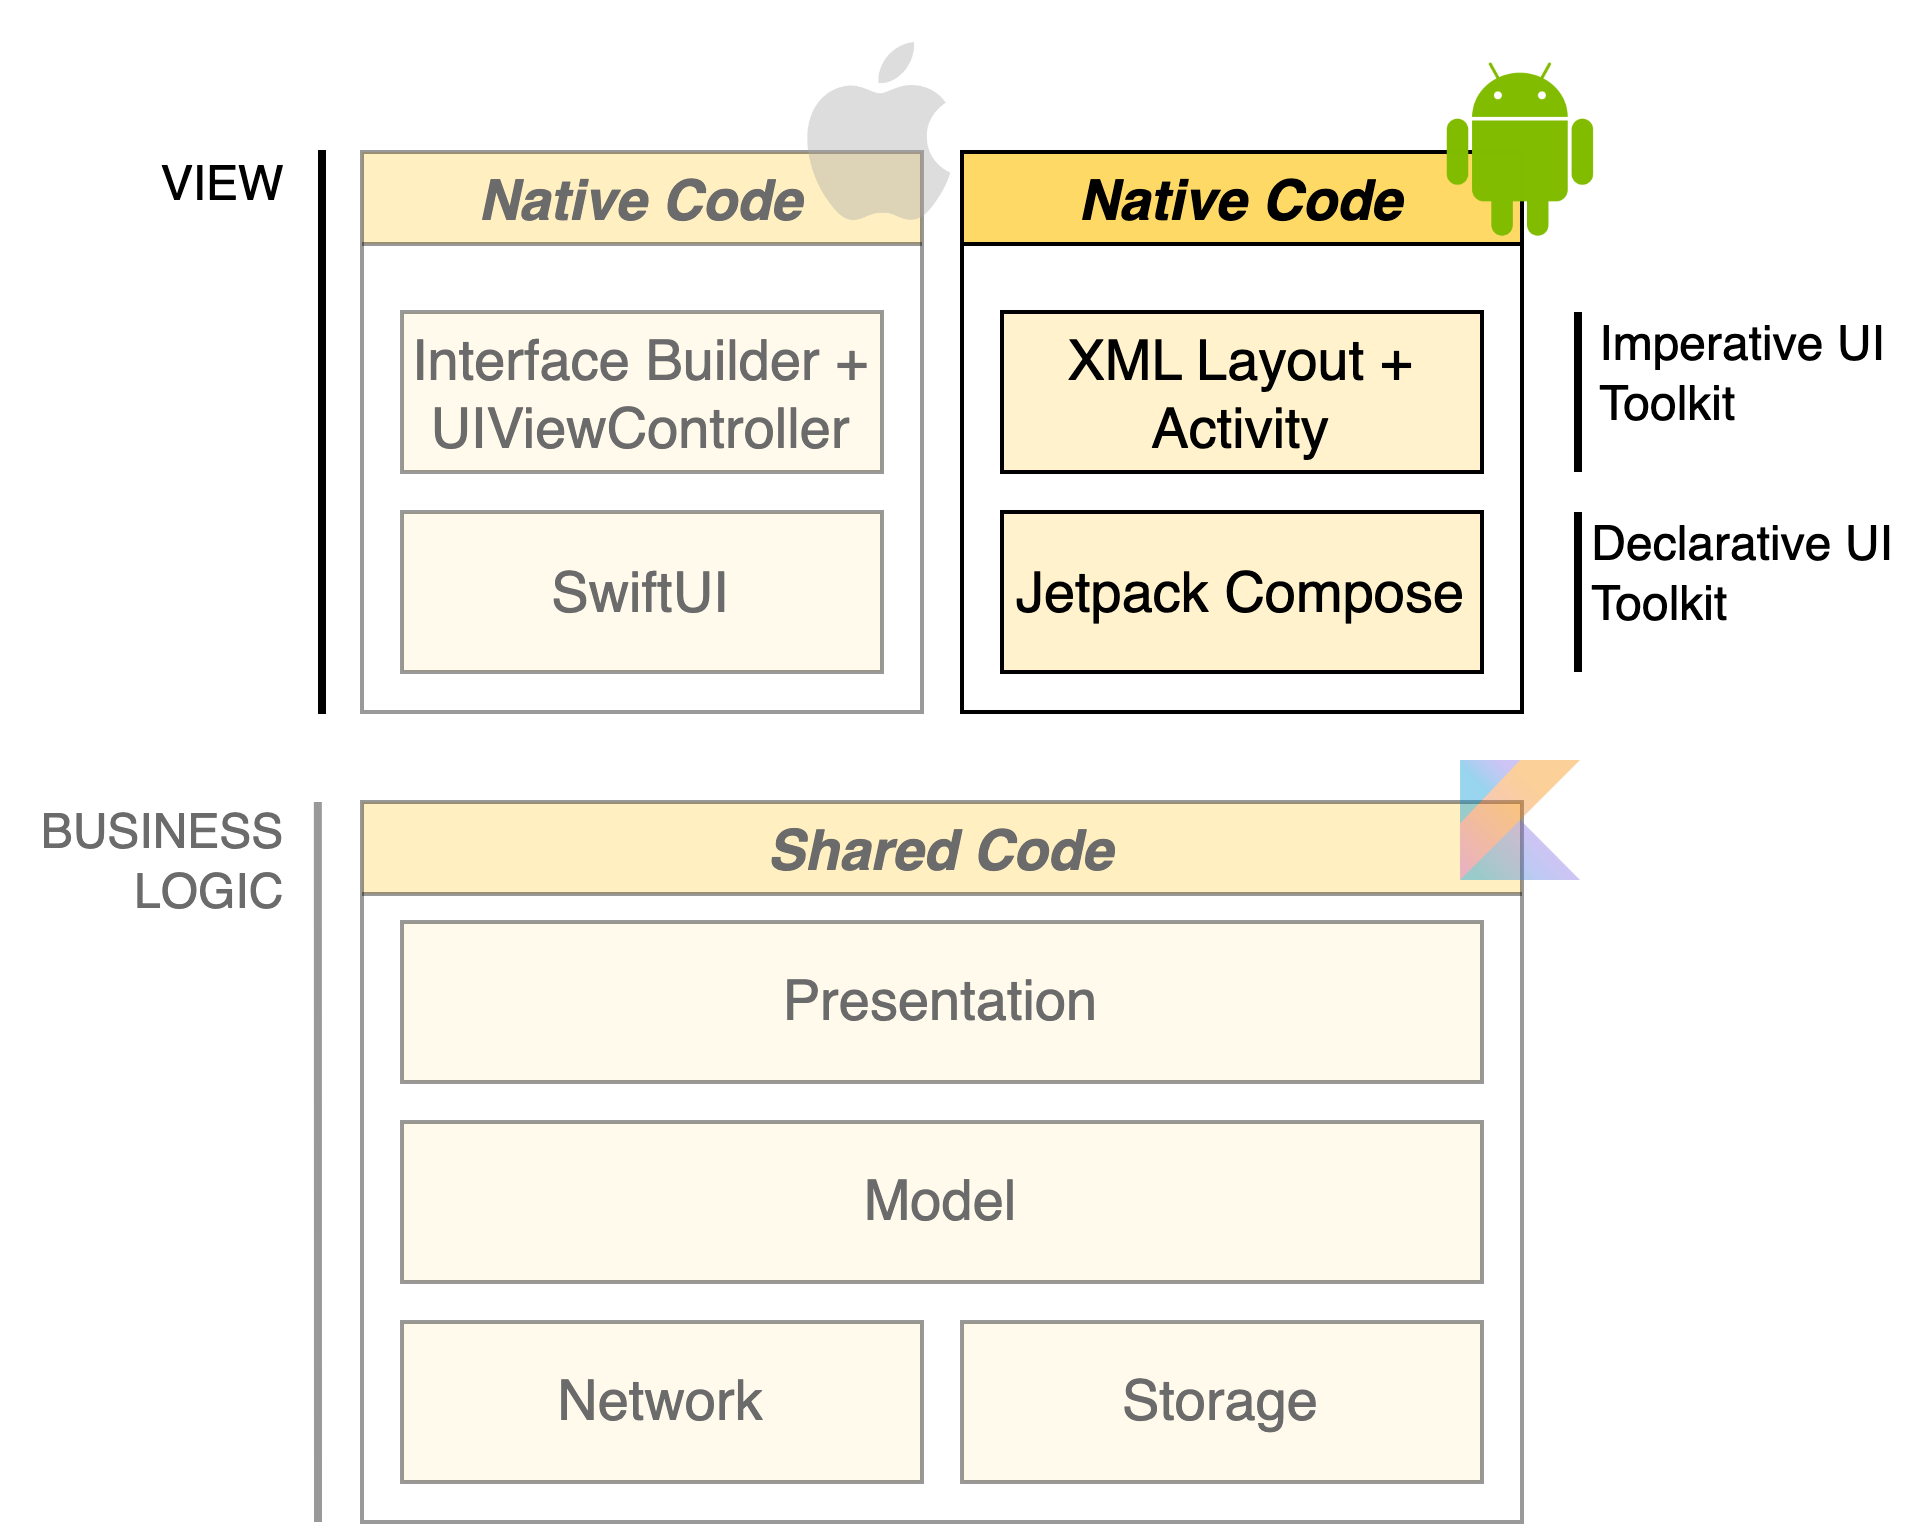
\includegraphics[width=1\textwidth]{img/stack_kmm_android.png}
            \end{figure}
        \end{column}
    \end{columns}
\end{frame}

\begin{frame}{UI Android}
    % citare readium kotlin
    \begin{columns}[onlytextwidth]
        \begin{column}{0.24\textwidth}
             \begin{figure}[H]
                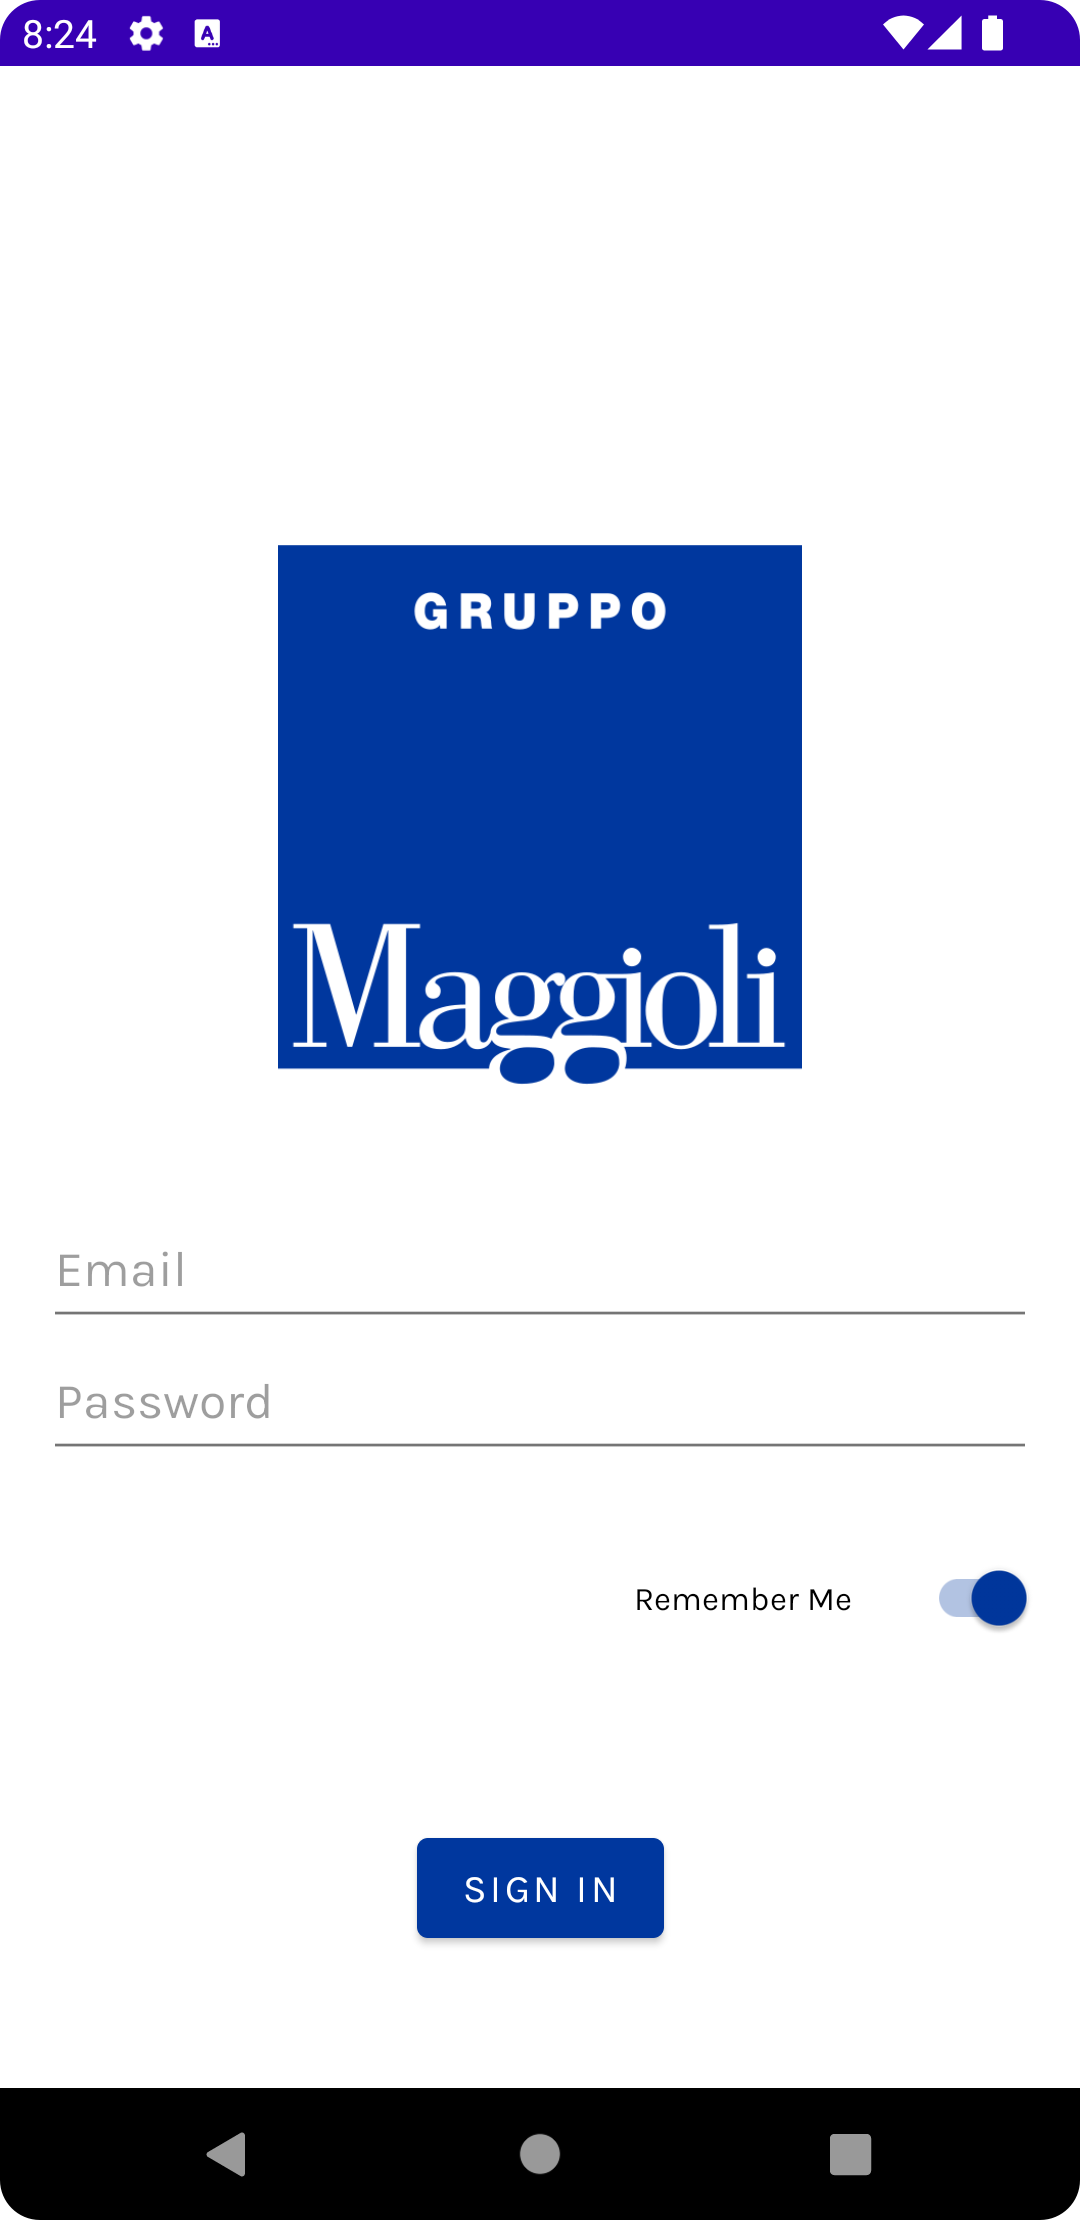
\includegraphics[width=1\textwidth]{img/login.png}
            \end{figure}
        \end{column}
        \begin{column}{0.24\textwidth}
             \begin{figure}[H]
                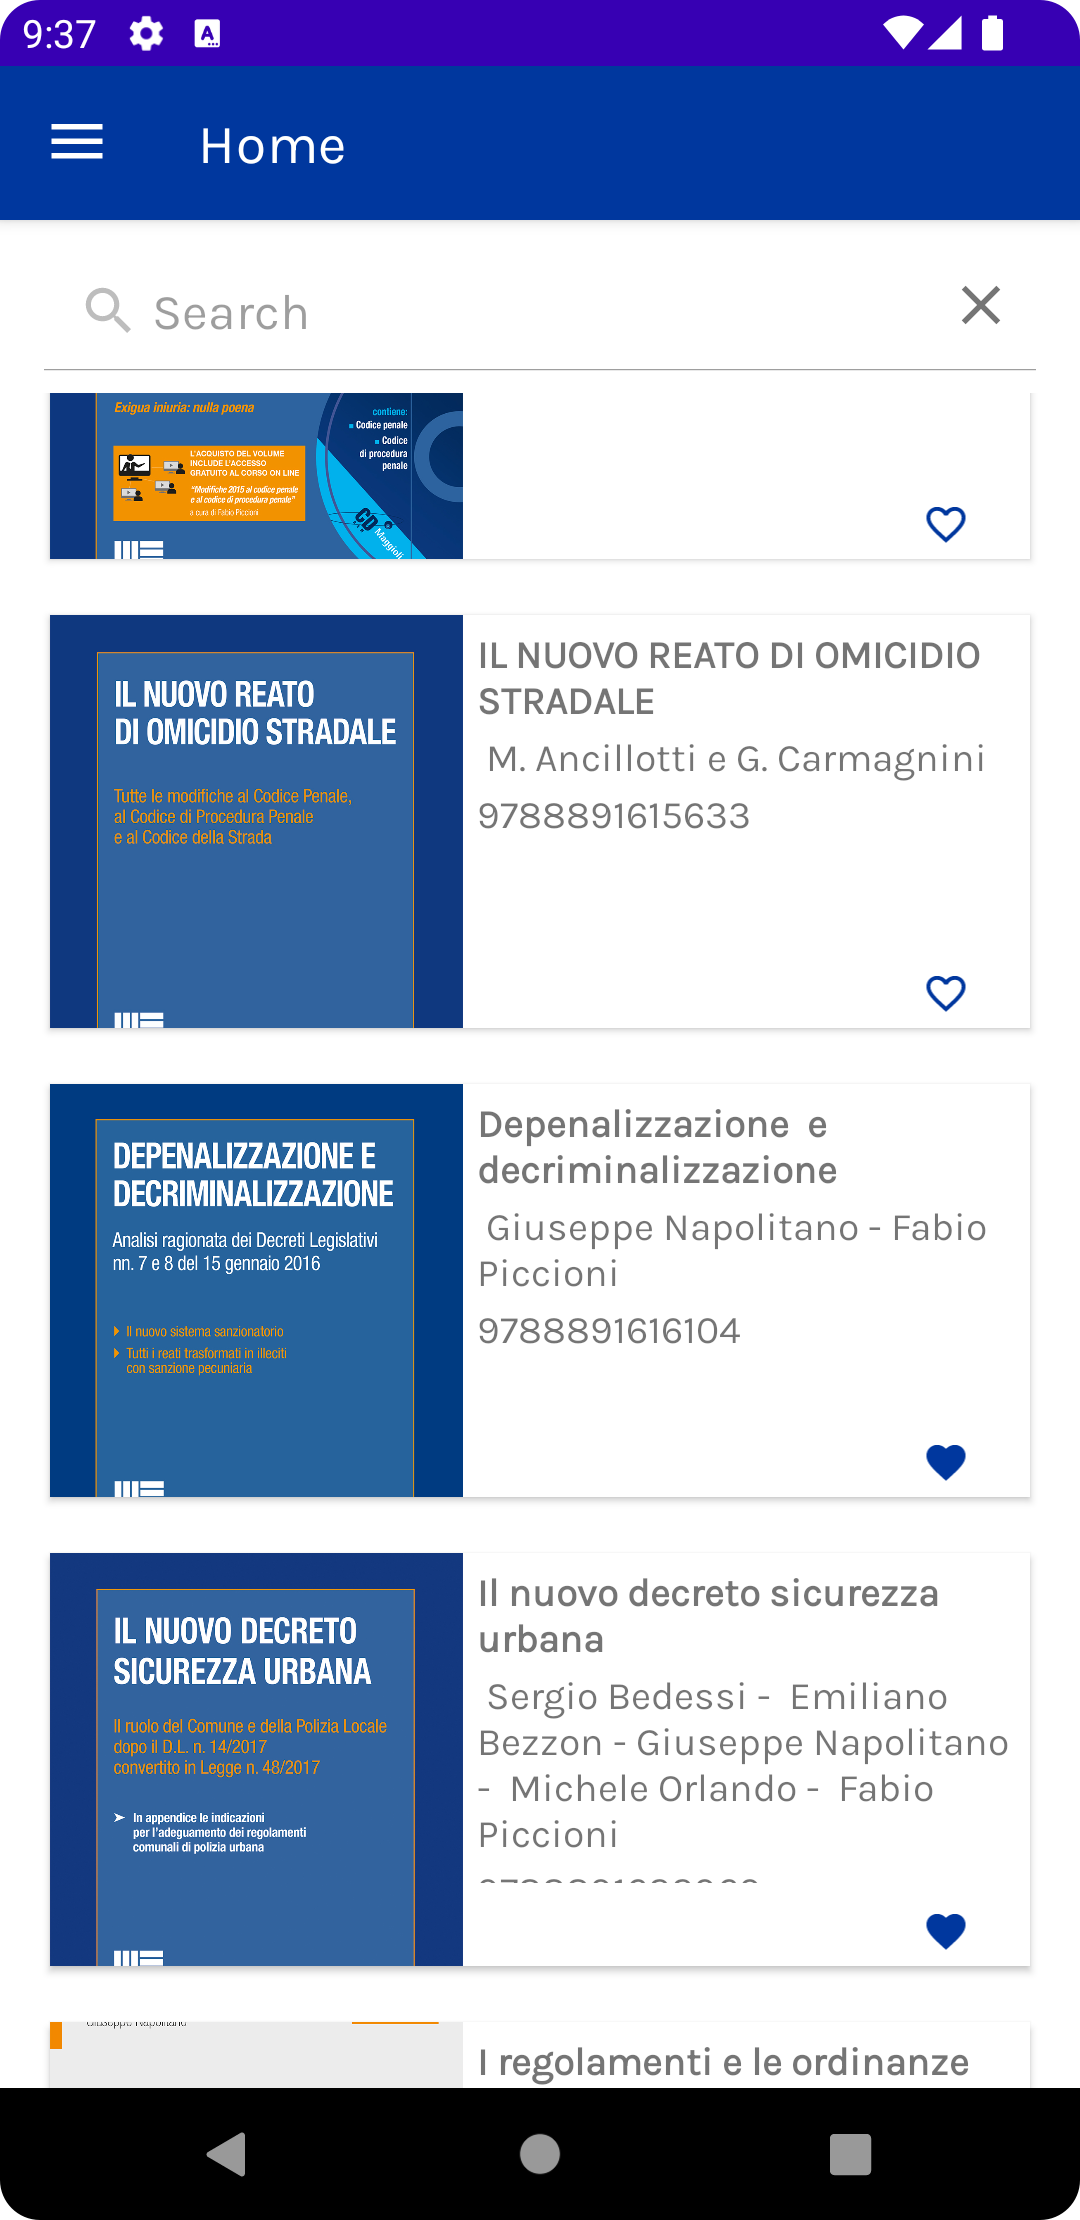
\includegraphics[width=1\textwidth]{img/home.png}
            \end{figure}
        \end{column}
        \begin{column}{0.24\textwidth}
             \begin{figure}[H]
                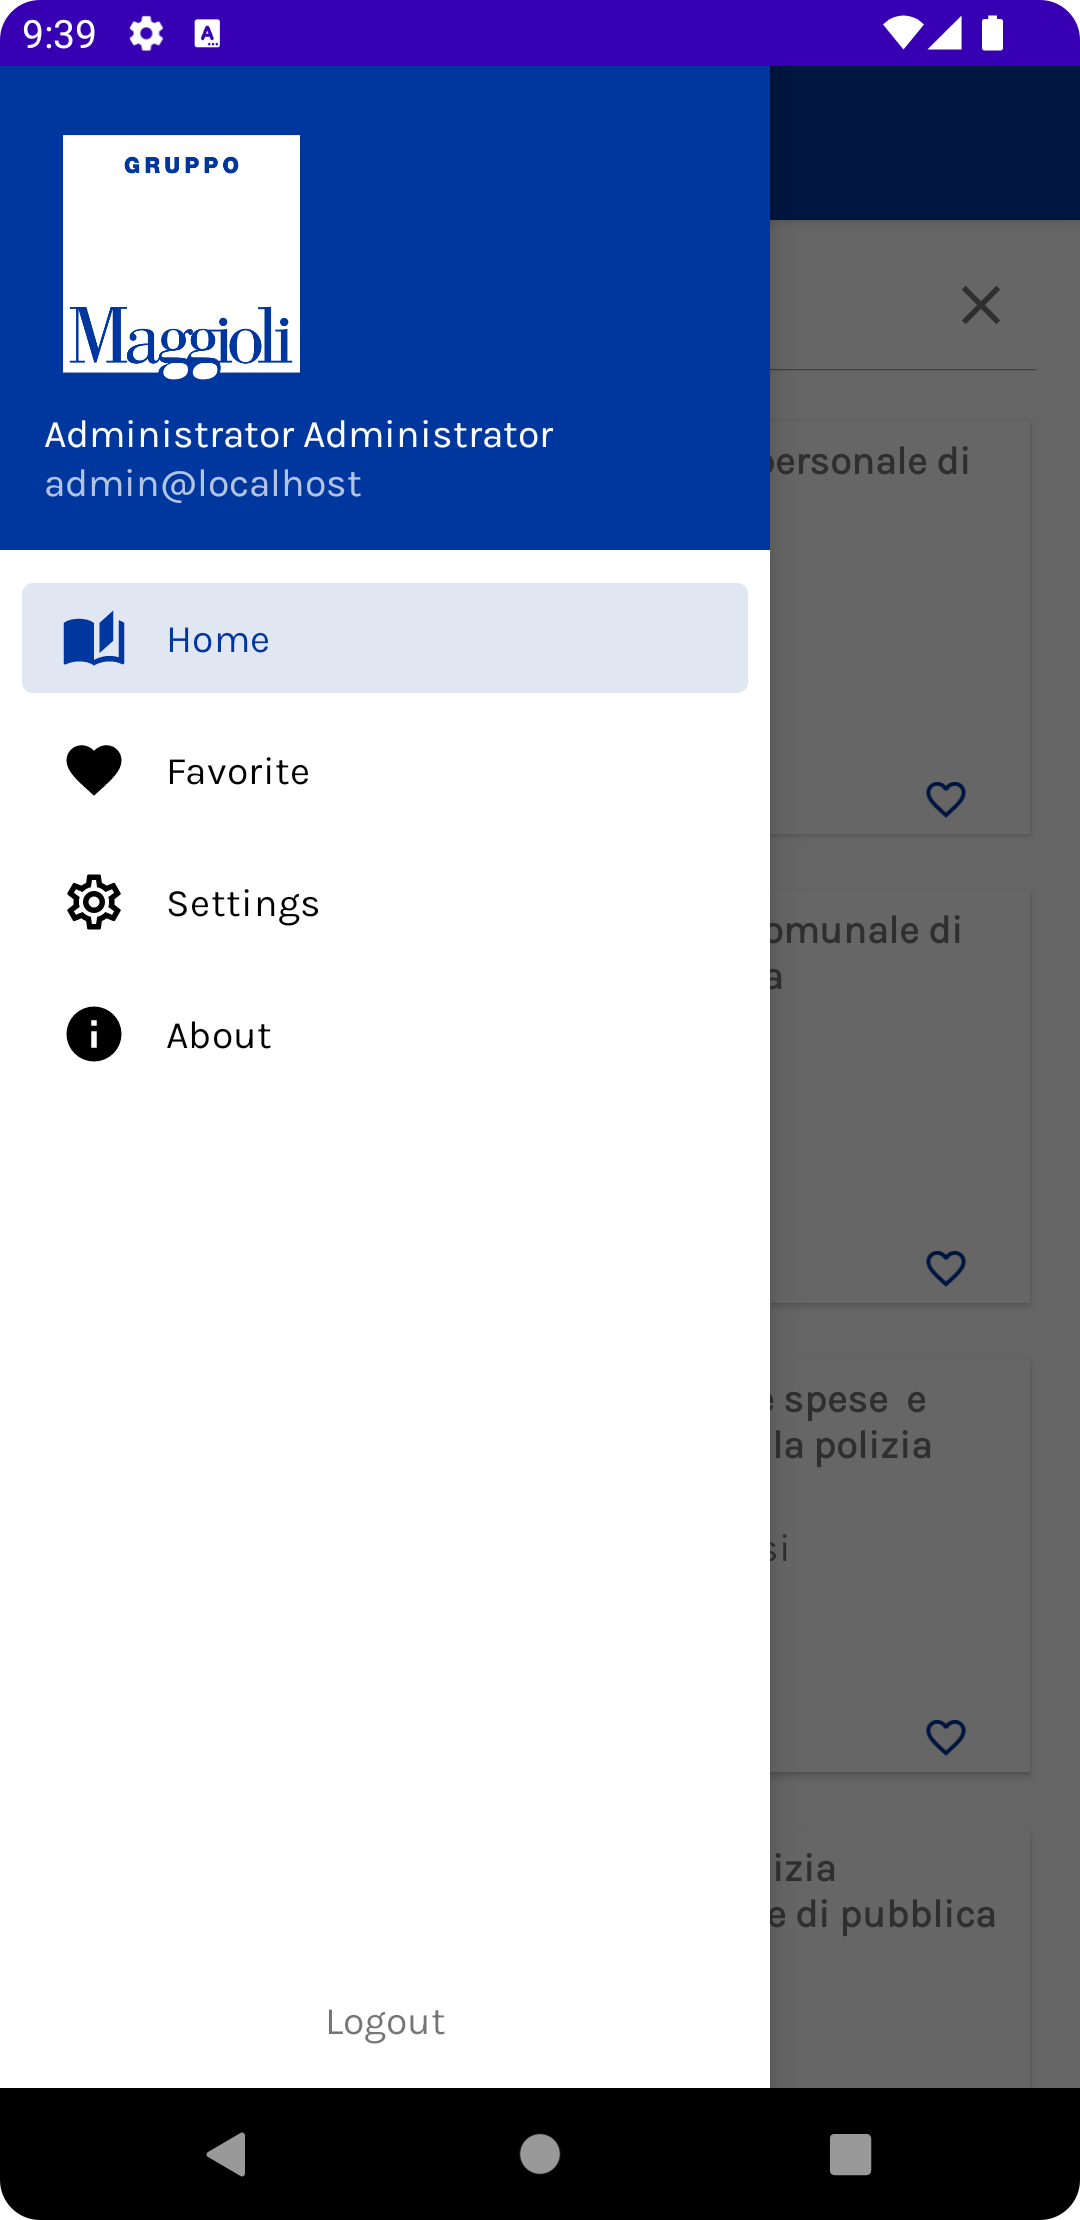
\includegraphics[width=1\textwidth]{img/sidenav.png}
            \end{figure}
        \end{column}
        \begin{column}{0.24\textwidth}
             \begin{figure}[H]
                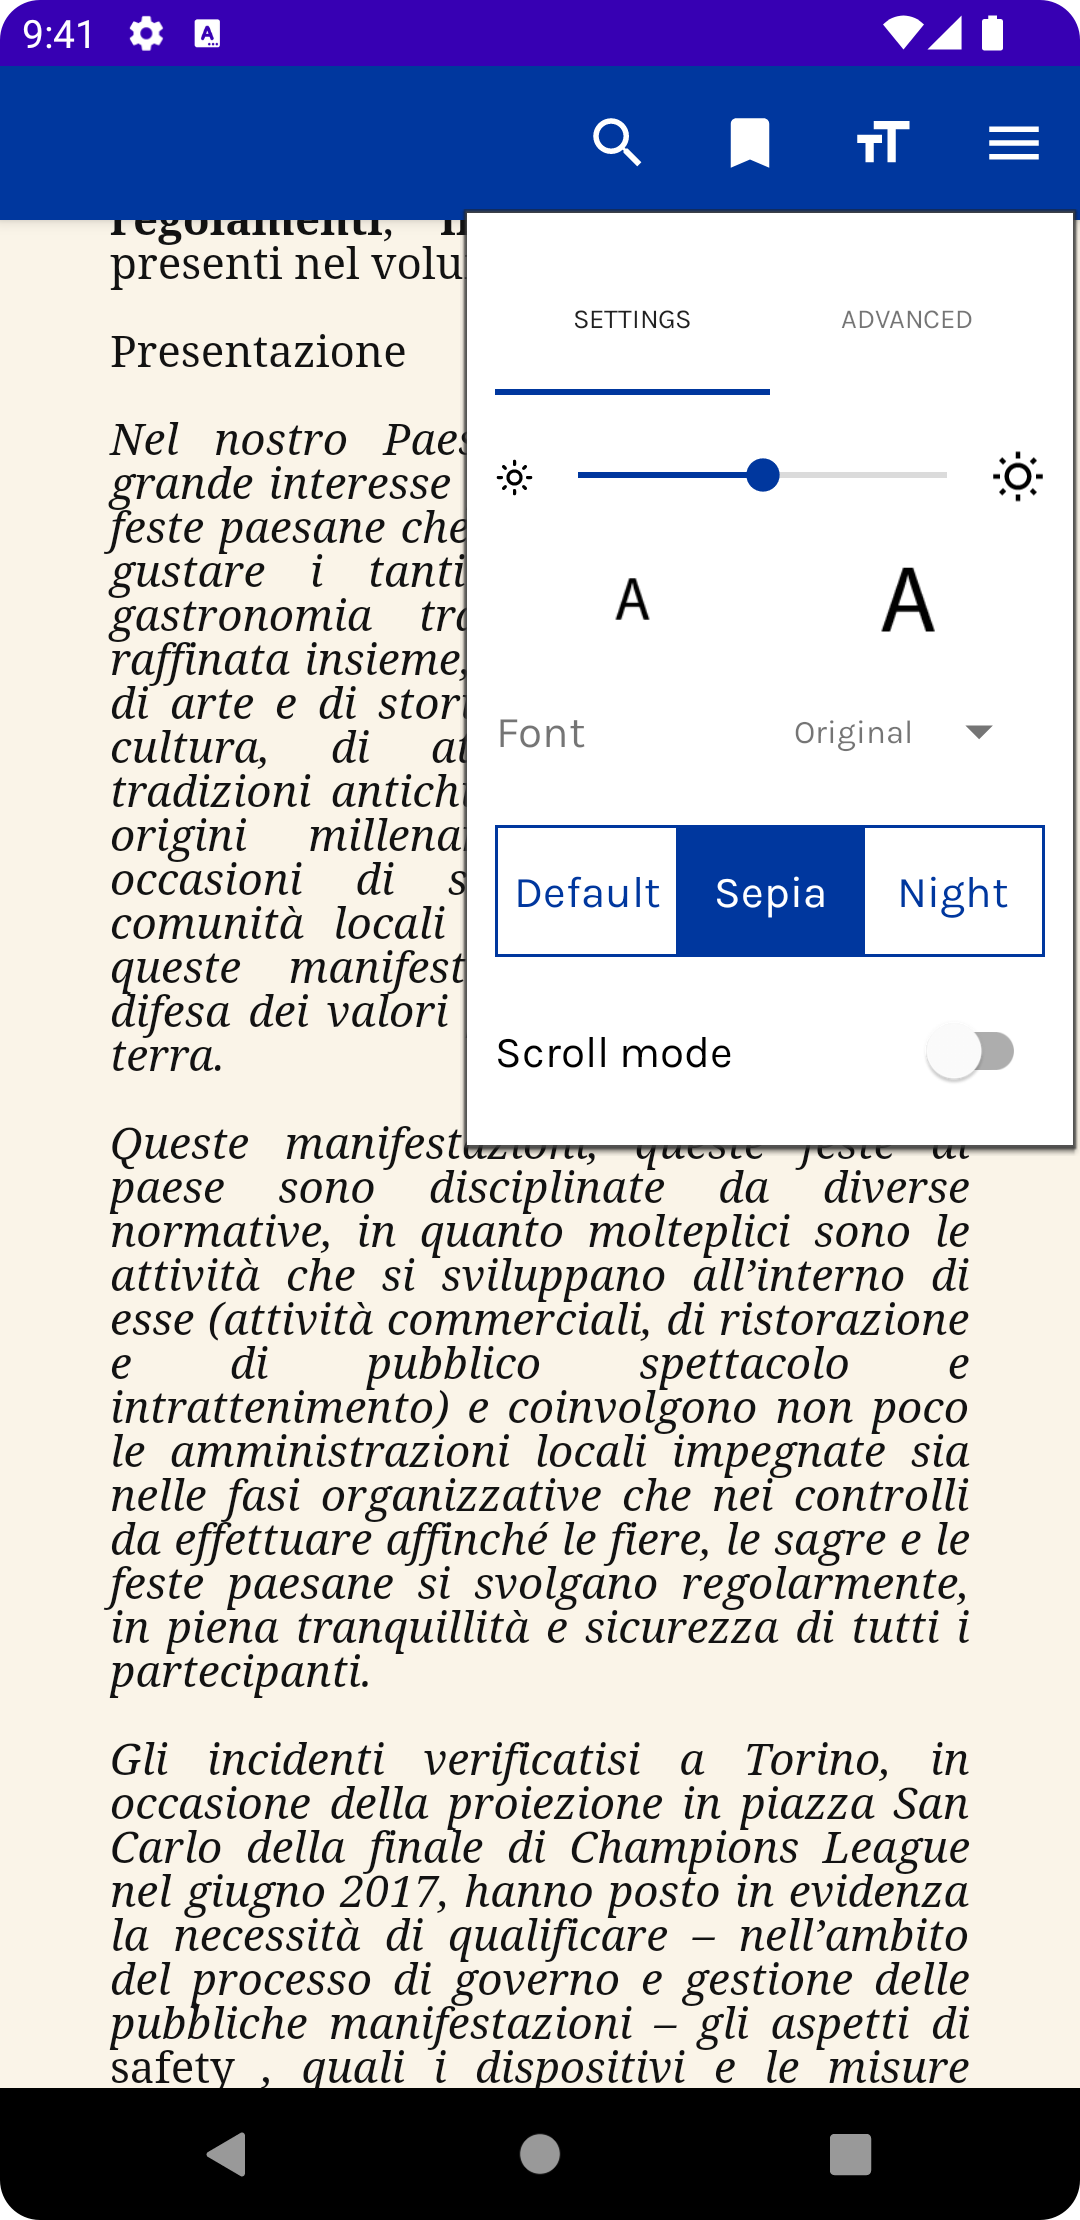
\includegraphics[width=1\textwidth]{img/reader_settings.png}
            \end{figure}
        \end{column}
    \end{columns}
\end{frame}

\begin{frame}{UI iOS}
    % citare readium swift
    \begin{columns}[onlytextwidth]
        \begin{column}{0.4\textwidth}

        \end{column}
        \begin{column}{0.6\textwidth}
             \begin{figure}[H]
                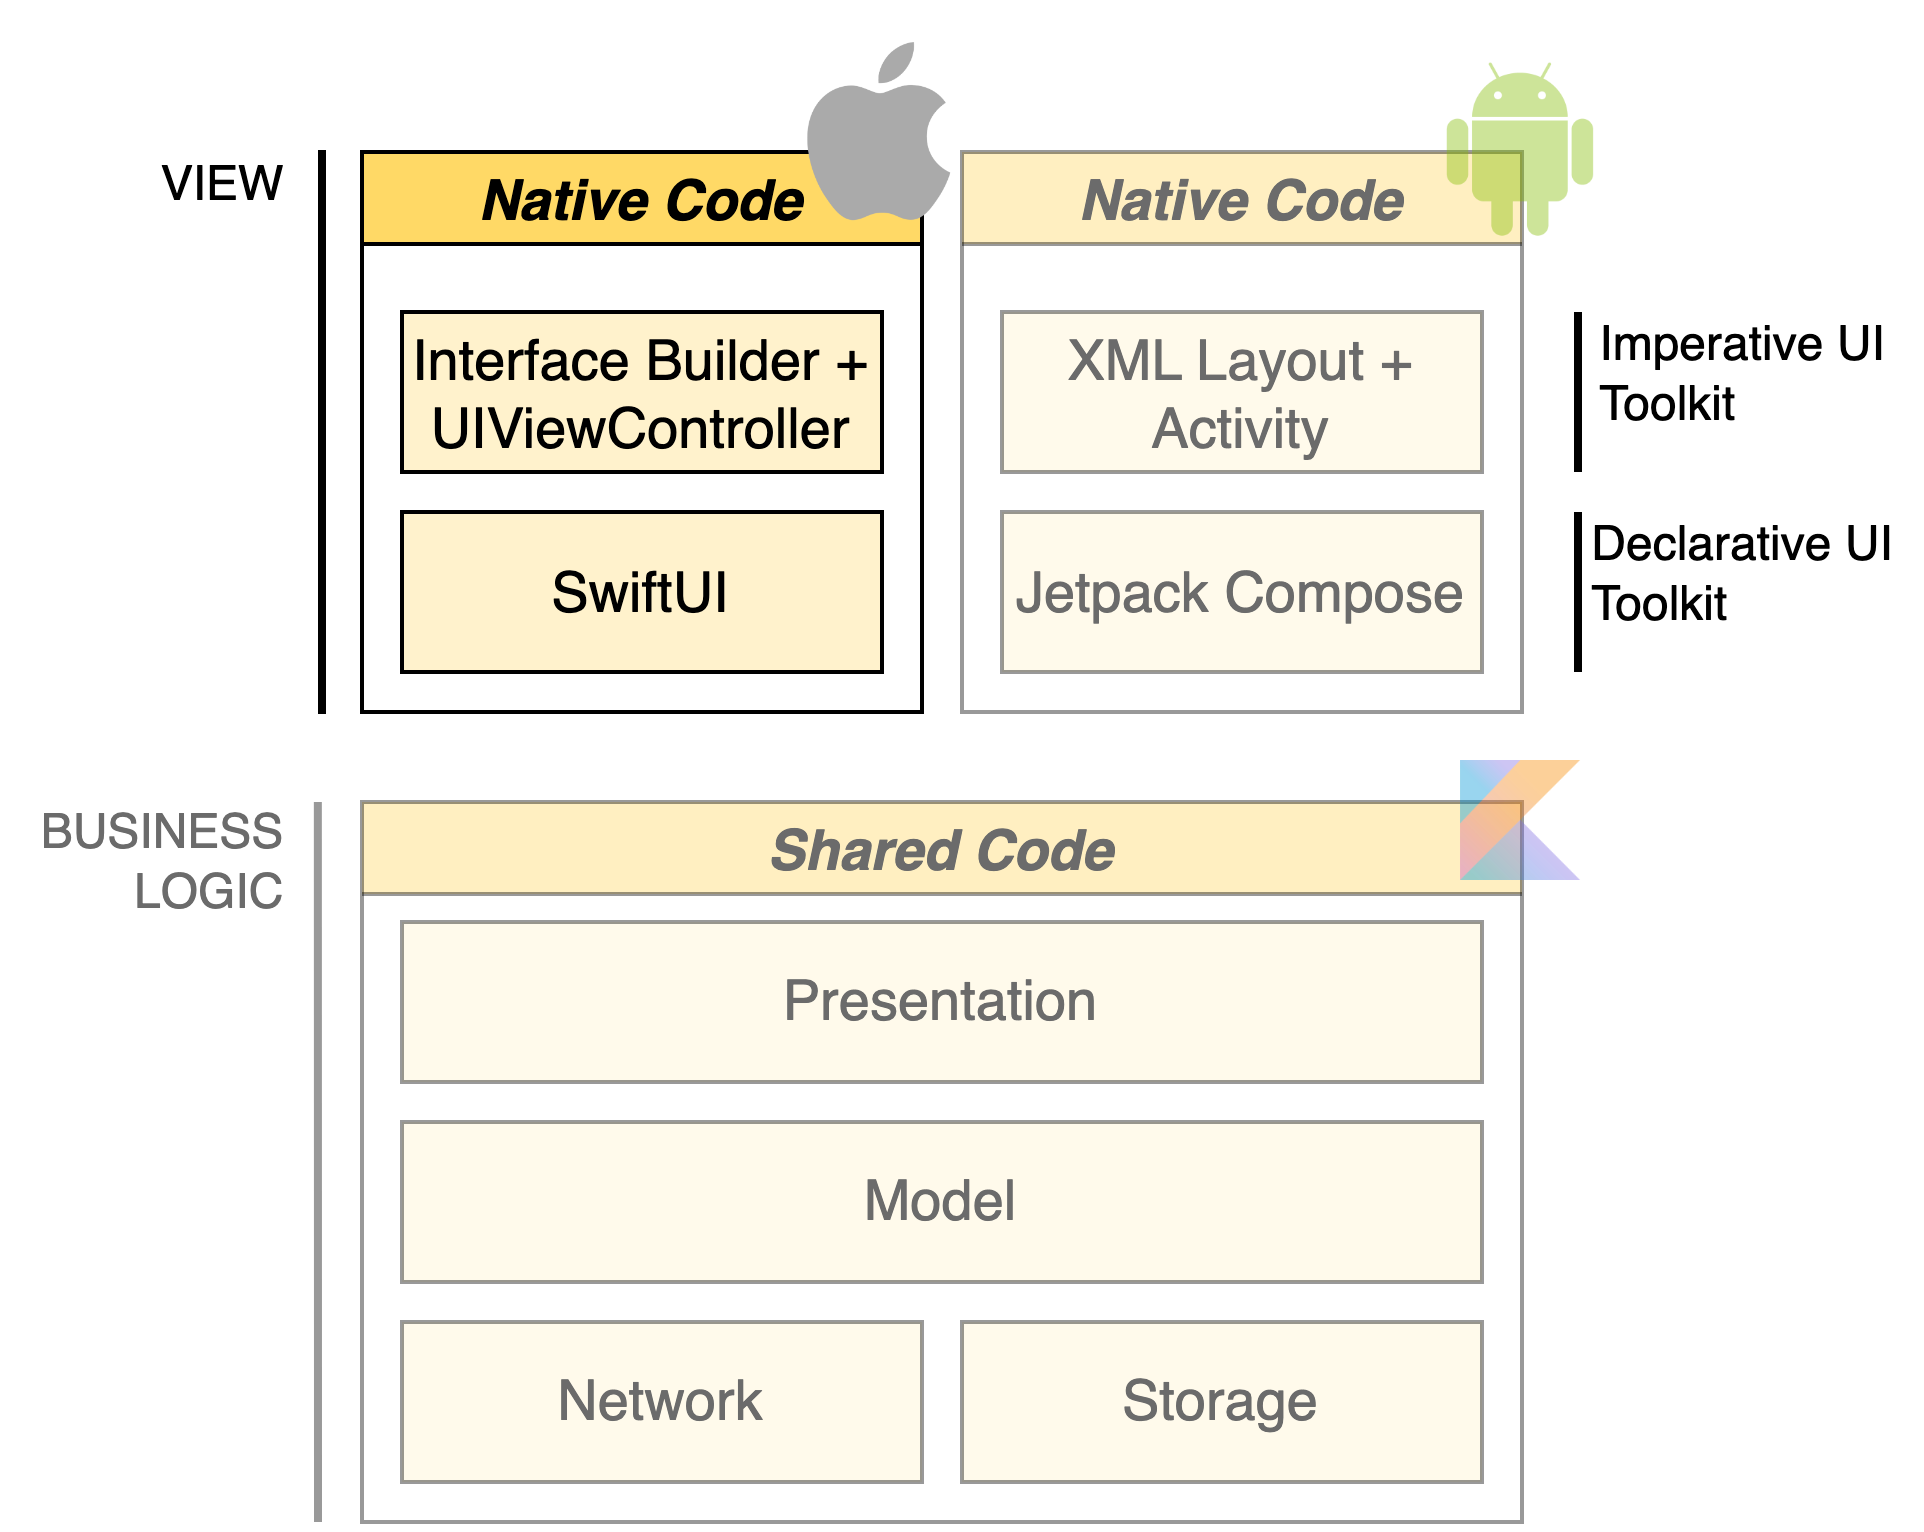
\includegraphics[width=1\textwidth]{img/stack_kmm_ios.png}
            \end{figure}
        \end{column}
    \end{columns}
\end{frame}

\begin{frame}{UI iOS}
    % citare readium kotlin
    \begin{columns}[onlytextwidth]
        \begin{column}{0.24\textwidth}
             \begin{figure}[H]
                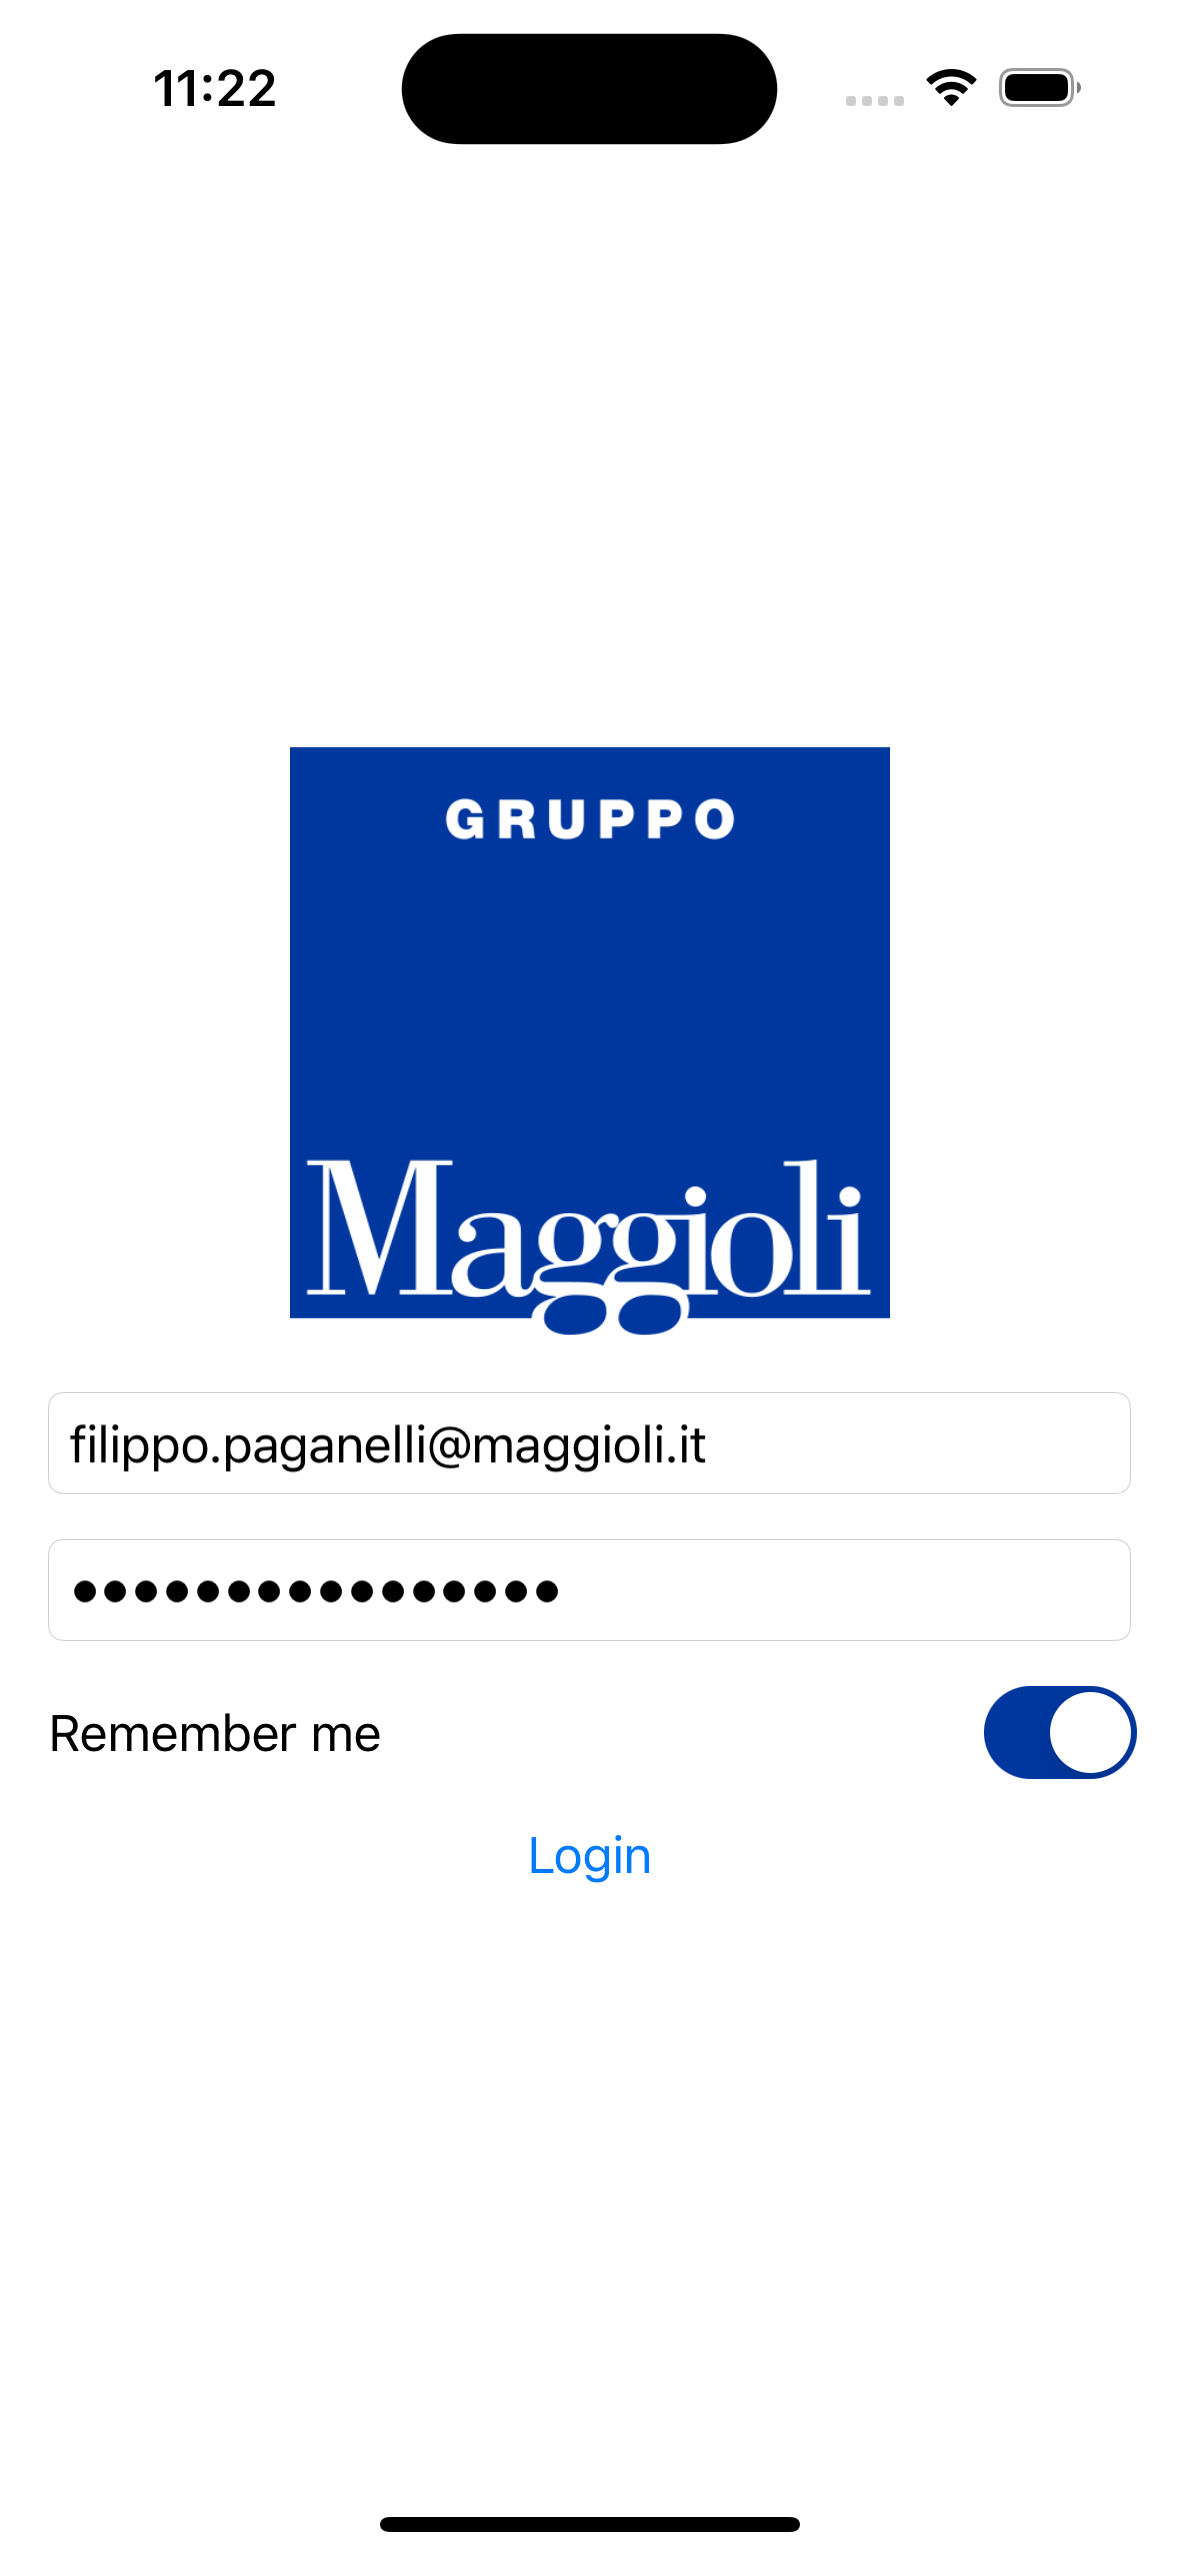
\includegraphics[width=1\textwidth]{img/login_ios.png}
            \end{figure}
        \end{column}
        \begin{column}{0.24\textwidth}
             \begin{figure}[H]
                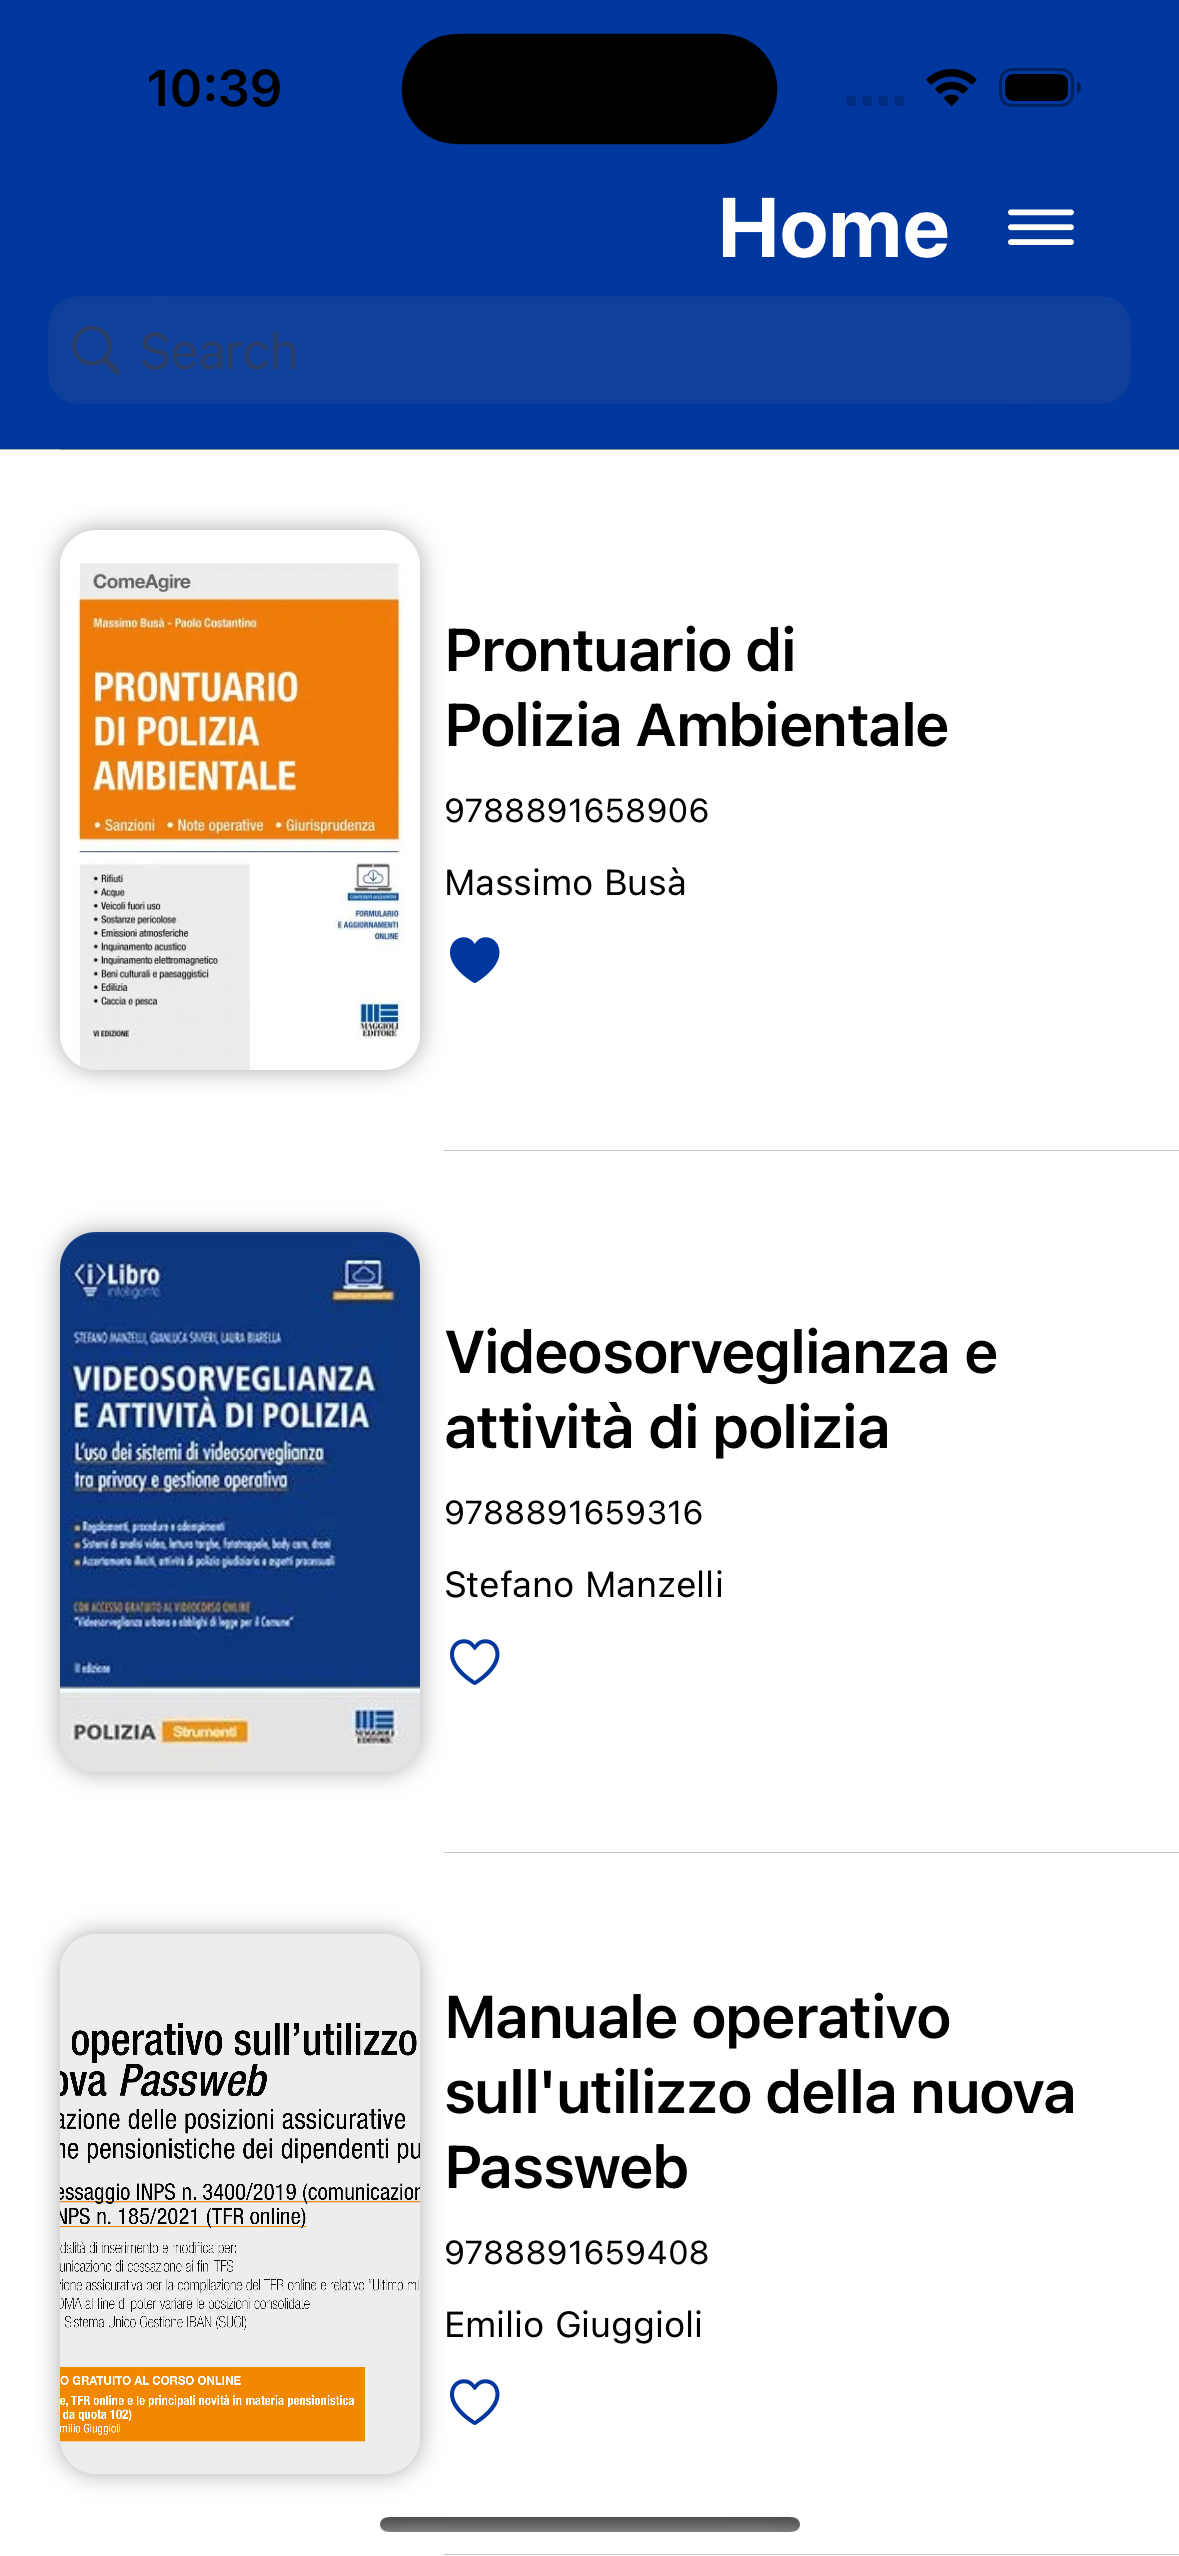
\includegraphics[width=1\textwidth]{img/home_ios.png}
            \end{figure}
        \end{column}
        \begin{column}{0.24\textwidth}
             \begin{figure}[H]
                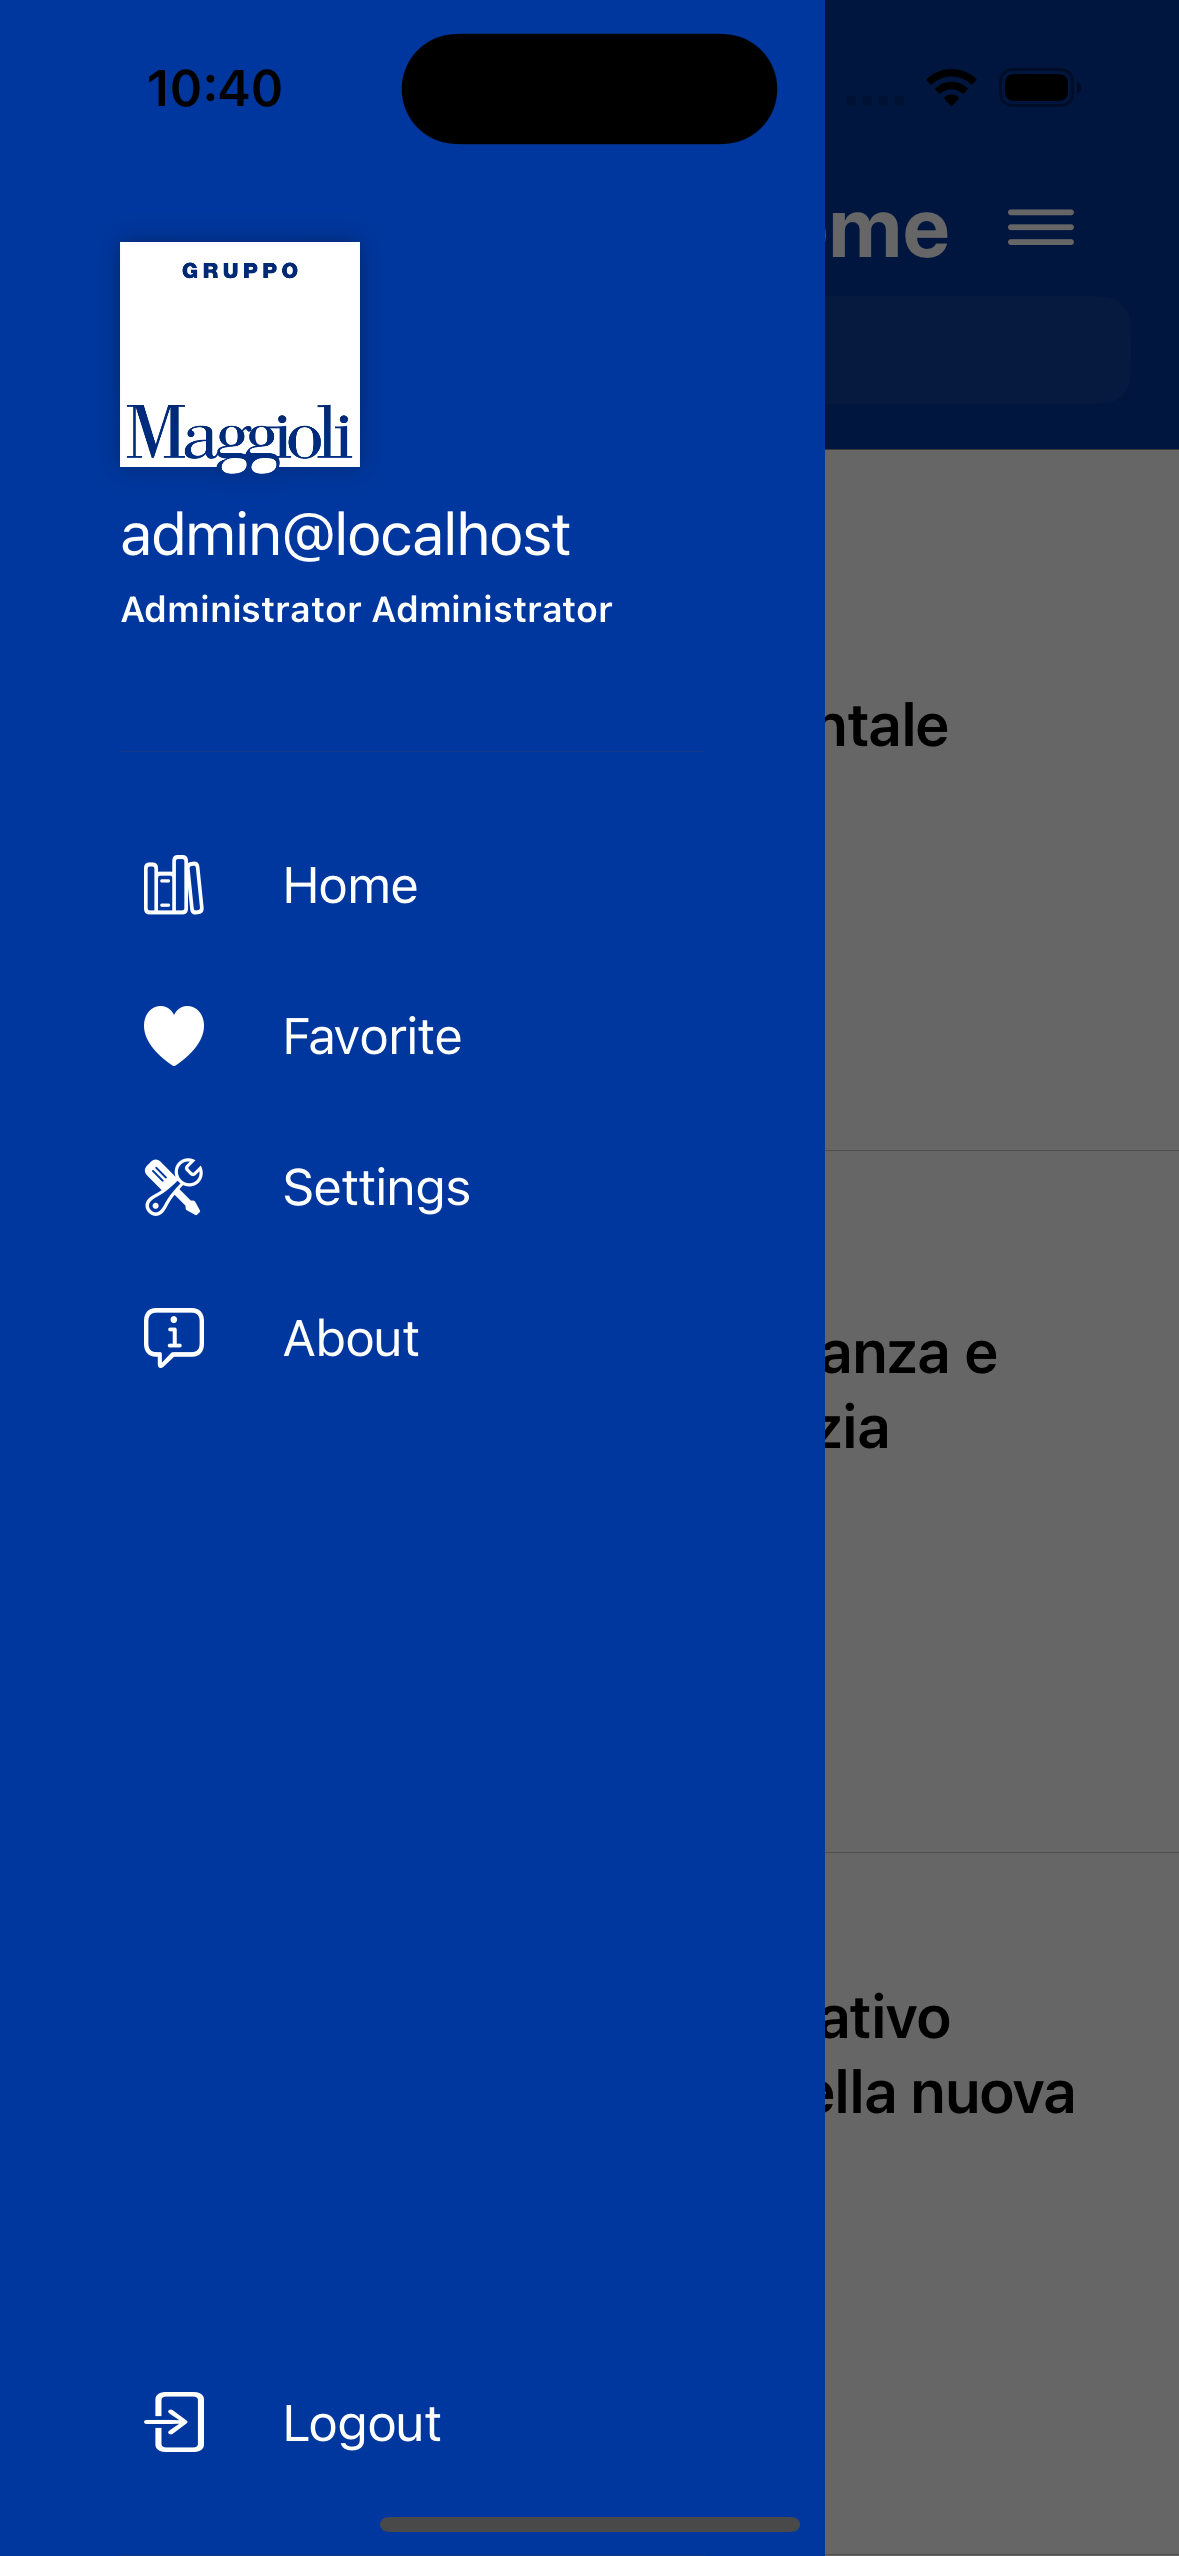
\includegraphics[width=1\textwidth]{img/sidenav_ios.png}
            \end{figure}
        \end{column}
        \begin{column}{0.24\textwidth}
             \begin{figure}[H]
                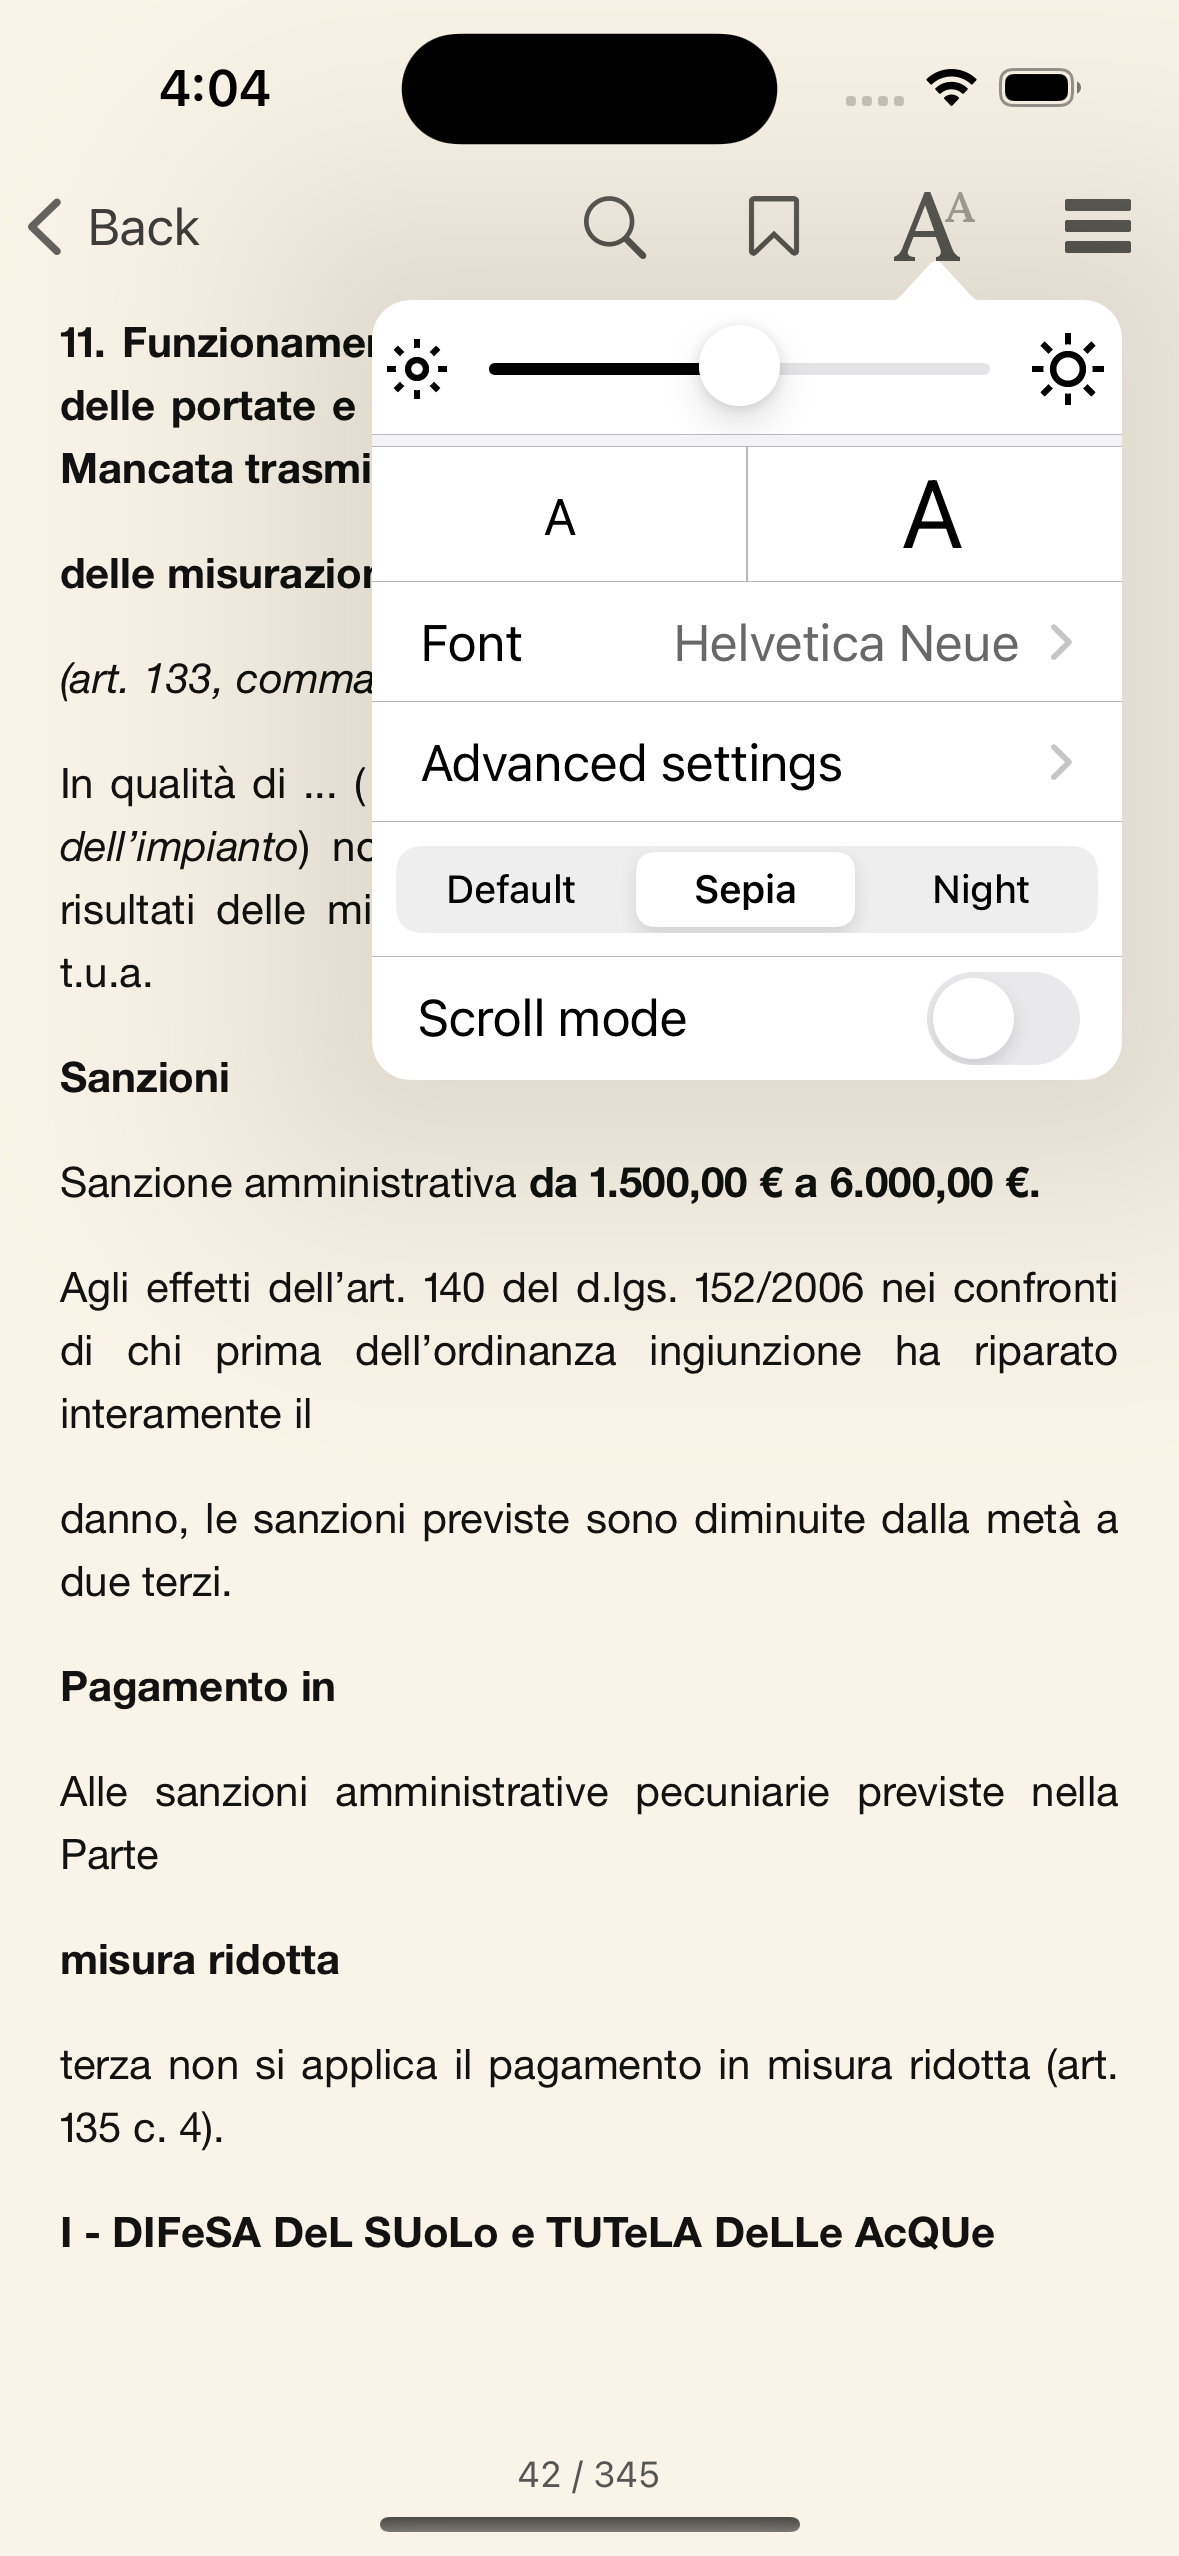
\includegraphics[width=1\textwidth]{img/reader_settings_ios.png}
            \end{figure}
        \end{column}
    \end{columns}
\end{frame}